\begin{frame}{Abstract}

	In my M.Sc. project, I study the effects of the backreaction of a charged Klein-Gordon
field coupled to an external electric field, in 1+1 dimensional spacetime.
In this talk, I summarize the statement of the problem I intend to solve, and present preliminary results and observations from my project. 
\end{frame}

\section{Preliminaries}
\begin{frame}{The set-up}
		    \begin{figure}[ht]
		        \centering
		        \incfig{the-background-field-generated-by-two-opposite-charges-sitting-at-the-boundaries.}
		        \caption{the background field generated by two opposite charges sitting at the boundaries.}
		        \label{fig:the-background-field-generated-by-two-opposite-charges-sitting-at-the-boundaries.}
		    \end{figure}
\end{frame}

%\begin{frame}{The vacuum solutions without background electric field}
%	\vspace{2cm}
%	\centering
%	\hspace{-2cm}$\lambda=0 \implies \rho(z) = 0$
%	\vspace{-2cm}
%\begin{figure}[ht]
%    \centering
%    \incfig{the-backreaction-of-the-klein-gordon-field.}
%    \caption{The background electric field and the free Klein-Gordon field.}
%    \label{fig:the-backreaction-of-the-klein-gordon-field.}
%\end{figure}
%\end{frame}

\begin{frame}{The set-up}
	\vspace{1cm}
	\centering
	\hspace{-2cm}$E\neq0 \implies \rho(z) \neq 0$
	\vspace{-1cm}
\begin{figure}[ht]
    \centering
    \incfig{the-backreaction-of-the-klein-gordon-field2}
    \caption{The backreaction of the Klein-Gordon field}
    \label{fig:the-backreaction-of-the-klein-gordon-field}
\end{figure}
\end{frame}

\begin{frame}
    \begin{themedTitleBlock}{Semi classical Klein-Gordon-Maxwell (KGM) equations}
	    \uncover<1->{
		    The goal is to solve the system of coupled differential equations
	            \begin{align*}
			    \begin{cases}
				    \left[ D_\mu D^\mu + m^2 \right] 	 \phi(t, z)= 0 
				    \\ 
				    \partial_\mu F^{\mu\nu} = j^{\nu}_\text{source} +  \left<j^{\nu} \right>_{\phi} 
			    \end{cases}
		    \end{align*}
		    \uncover<2->{
		        With the gauge covariant derivative $$D_\mu = \partial_\mu + ieA_\mu,$$ } } \uncover<3->{
				\hspace{-0.3cm}and the boundary conditions
	        \begin{align*}
	        	\begin{cases}
				\left . \hspace{0.14cm}\phi\hspace{0.9mm} \right|_{z=0, 1} &= 0 \\
					\left . F^{\mu\nu}\right|_{z=0, 1} &= \lambda 
	        	\end{cases}
	        \end{align*}
	    }
    \end{themedTitleBlock}
\end{frame}

\begin{frame}{Gauge fixing}
	\begin{columns}
	    \begin{column}{0.5\textwidth}
\begin{figure}[ht]
    \centering
    \incfig{the-background-classical-electric-field-and-potential}
    \caption{The background electric potential}
    \label{fig:the-background-classical-electric-field}
\end{figure}
	    \end{column}
	    \begin{column}{0.5\textwidth}
		    \begin{enumerate}[<+->]
		    	\item 
	    Constant electric field of strength $\lambda$ pointing towards positive $z.$
    \item Under the Coulomb gauge $$A_0(t, z) = -E z,\, A_1(t, z) = 0$$ up to additive constant
    \item To ensure anti-symmetric solutions $$A_0(t, z)=-E(z-\frac{1}{2})$$

		    \end{enumerate}
	    \end{column}
	\end{columns}

\end{frame}
\begin{frame}{Gauge fixing}

	\begin{columns}
	    \begin{column}{0.5\textwidth}
\begin{figure}[ht]
    \centering
    \incfig{the-background-electric-field-and-potential,-with-an-additional-(antisymmetric)-potential.}
    \caption{The full electric potential (background+backreaction)}
    \label{fig:the-background-classical-electric-field}
\end{figure}
	    \end{column}
	    \begin{column}{0.5\textwidth}
		    \begin{enumerate}
		    	\item 
	    Constant electric field of strength $\lambda$ pointing towards positive $z.$
    \item Under the Coulomb gauge $$A_0(t, z) = -E z,\, A_1(t, z) = 0$$ up to additive constant
    \item To ensure anti-symmetric solutions 
	    \begin{align*}
	    	A_0(t, z)=-E(z-\frac{1}{2}) \\ + A_0^{\text{br}}(z)
	    \end{align*}

		    \end{enumerate}
	    \end{column}
	\end{columns}

\end{frame}

\begin{frame}{The set up}
	\begin{themedTitleBlock}{Klein-Gordon equation}
		With the chosen gauge the KGM equations turn into
	\begin{align*}
		( (\partial_t + ie A_0) ^2 - \partial_z^2+ m^2) \phi (t, z) &= 0,\\ 
		\partial_z ^2 A_0^{^{br}} &= - \left<\rho (z) \right>_\phi,
	\end{align*}
with  
\begin{align*}
	A_0 (z) &= -E\left( z - \frac{1}{2} \right) + A_0^{\text{br}}(z), \\
	\rho(z) &=  ie \left( (D_0 \phi) ^* \phi - \phi^* D_0\phi \right)
\end{align*}
	\end{themedTitleBlock}
\end{frame}

\begin{frame}{Time independent Klein-Gordon equation}
	\begin{themedTitleBlock}{Mode equation}
		    \begin{align*}
\uncover<1->{
    \phi(t, z) = \phi_n(z)e^{-i\omega_n t} \implies 
}
\uncover<2->{
    \left( \left[ \omega_n - eA_0(z)  \right]^2 + \frac{d^2}{d z ^2} - m^2  \right) \phi_n &= 0 
}
		    	\end{align*}
			\uncover<3->{
				Ignoring the backreaction of the scalar field \alert{(External field approximation)}
			    	\begin{align*}
			    	\left( \left[ \omega_n + \lambda \left(  z - \frac{1}{2}\right)  \right]^2 + \frac{d^2}{d z ^2}  - m^2\right) \phi_n &= 0, \,\,\, \lambda = eE
			    \end{align*}
			}
	\end{themedTitleBlock}
\end{frame}

\section*{External field approximation}

\begin{frame}{Analytic solutions}
	When $A_0(z) = -\lambda (z-\frac{1}{2})$, the KG equation can be solved analytically
\begin{align*}
	\phi_n(z) &= 
	a_n D_{i \frac{m^2}{2\lambda} - \frac{1}{2}} \left( 
		\frac{1+i}{\sqrt{\lambda} }
		\left( \omega_n + \lambda \left( z-\frac{1}{2} \right)
		\right) 
	\right) 
	\\
		  &+
	b_n D_{-i \frac{m^2}{2\lambda} - \frac{1}{2}} \left( 
		\frac{i - 1}{\sqrt{\lambda} }
		\left( \omega_n + \lambda \left( z-\frac{1}{2} \right)
		\right) 
	\right)
	\label{eq:parabolyc-cylinder}
\end{align*}
with $D_\nu(z)$ the parabolic cylinder functions.
\end{frame}

\begin{frame}{Instabilities of the external field approximation}
	The external field approximation yields instabilities for critical $\lambda$ values \cite{Ambj1983}:
	\begin{figure}[h]
		\centering
		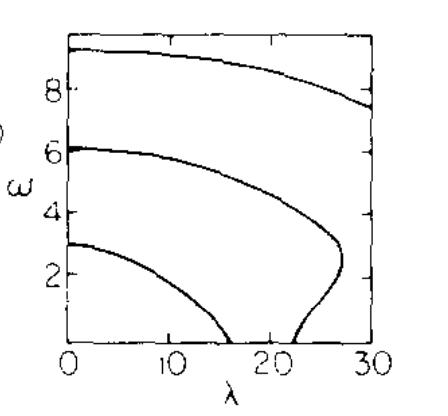
\includegraphics[width=0.4\textwidth]{figures/omega_wolfram.jpeg}
		\caption{Energy of the first three modes as the background field strength  $\lambda$ increases, without considering the backreaction of the field. Courtesy of \cite{Ambj1983}. }
		\label{fig:figures-complex-eigenvalues-png}
	\end{figure}
\end{frame}

\begin{frame}{Backreaction avoids those instabilities?}
	The main claim in \cite{Ambj1983} is that considering the backreaction of the scalar field raises the energy levels, avoiding instabilities
	   \begin{figure}[h]
	   	\centering
	   	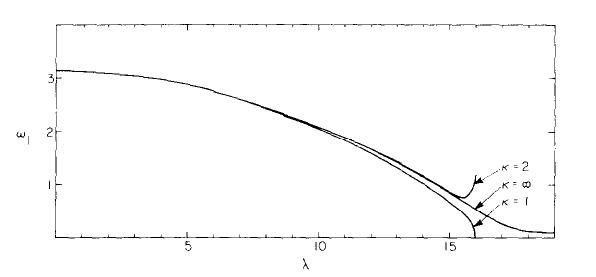
\includegraphics[width=0.8\textwidth]{figures/omega_backreaction.jpeg}
		\caption{Positive energy levels for increasing $\lambda$ \textbf{with} backreaction considered. \cite{Ambj1983}}
	   	\label{fig:figures-omega_backreaction-jpeg}
	   \end{figure} 
\end{frame}

\section*{Quantisation and renormalisation}

\begin{frame}{Vacuum polarization}
	Vacuum polarization is calculated as the zeroth component of the charge density current
\begin{align*}
	\rho(z) = ie \left( \left( D_0 \phi\right)^*\phi  - \phi^* D_0\phi\right).
\end{align*}

This operator is non-linear on the fields $\implies$ ill-defined expectation value. 

\end{frame}

%\begin{frame}{Quantization}
%The general solution (after quantization) to the Klein-Gordon equation can be written as 
%\begin{align*}
%	\phi(t, z) = \sum_{n>0}^{} a_n \phi_n(z) e^{-i\omega_nt}
%	+\sum_{n<0}^{} b_n^{\dagger} \phi_n(z) e^{-i\omega_nt},
%\end{align*}
%with $a_n$, and $b_n$ operators obeying 
%\begin{align*}
%	[a_n, a^\dagger_m] = [b_n, b^\dagger_m] = \delta_{nm}
%\end{align*} 
%and all other commutators vanishing.
%
%In our case, this defines the vacuum as 
%\begin{align*}
%	a_n\ket{0_\lambda} =
%	b_n\ket{0_\lambda} = 0 
%\end{align*}
%\end{frame}

\begin{frame}{Mode expansion of the vacuum polarization }
	In \cite{Ambj1983} the vacuum polarization is directly calculated as 
\begin{align*}
	\begin{split}
		&\bra{0} \rho(z) \ket{0}  = ie \bra{0}  \phi^* D_0\phi- \phi \left( D_0\phi \right) ^*  \ket{0} = \\
					 &	e \left( 
		    			 \sum_{n>0}^{} (\omega_n - eA_0) \lvert \phi_n  \rvert ^2
					+\sum_{n<0}^{} (\omega_n - eA_0) \lvert \phi_n  \rvert ^2
		    		\right)
	\end{split}
\end{align*}
\end{frame}

\begin{frame}{Hadamard states}
	Assume the two-point function $w(x, x')$ is of Hadamard form
\begin{align*}
	\bra{0} \phi(x)\phi^*(x') \ket{0} = w(x, x') = \underbrace{H(x, x')}_\text{Divergent}+ \underbrace{R(x, x')}_\text{Smooth}
\end{align*}

\uncover<2->{
    $w(x, x')$ is a divergent distribution as $x'\to x$, but so is $H(x, x')$. In a way similar to the normal ordering prescription of RQFT, define
    \begin{align*}
    	\bra{0} D_\alpha \phi (x) \left( D_\beta \phi(x) \right)^*  \ket{0} := \lim_{x' \to x} \left[ D_\alpha D'^*_{\beta'} \left( w(x, x') - H(x, x') \right)  \right] .
    \end{align*}
}

\end{frame}


\begin{frame}{Renormalized vacuum polarization}
	\uncover<1->{
	    	\begin{themedTitleBlock}{Hadamard Point-splitting\cite{Wern2020}}
	    \begin{align*}
	    	\begin{split}
	    		&\bra{0} \rho(z) \ket{0}  = ie \bra{0}  \phi^* D_0\phi- \phi \left( D_0\phi \right) ^*  \ket{0} = \\
	    					 &	e \lim_{\tau \to 0}\left( 
	    		    			 \sum_{n>0}^{} (\omega_n - eA_0) \lvert \phi_n  \rvert ^2e^{i\omega_n(\tau +i\epsilon)}  
	    					+\sum_{n<0}^{} (\omega_n - eA_0) \lvert \phi_n  \rvert ^2e^{-i\omega_n(\tau +i\epsilon)} 
	    		    		\right)
	    		    		+ \frac{e^2}{\pi}A_0
	    	\end{split}
	    \end{align*}
	    
	    	\end{themedTitleBlock}
	}
	
	\uncover<2->{
	    
	\begin{themedTitleBlock}{Mode sum formula \cite{Ambj1983}}
\begin{align*}
	\begin{split}
		&\bra{0} \rho(z) \ket{0}  = ie \bra{0}  \phi^* D_0\phi- \phi \left( D_0\phi \right) ^*  \ket{0} = \\
					 &	e \left( 
		    			 \sum_{n>0}^{} (\omega_n - eA_0) \lvert \phi_n  \rvert ^2
					+\sum_{n<0}^{} (\omega_n - eA_0) \lvert \phi_n  \rvert ^2
		    		\right)
	\end{split}
\end{align*}
	\end{themedTitleBlock}

	}
\end{frame}
\begin{frame}{Renormalized vacuum polarization}
	    	\begin{themedTitleBlock}{Hadamard Point-splitting\cite{Wern2020}}
	    
\begin{align*}
	\begin{split}
		\bra{0} \rho(z) \ket{0}  = 
					 	e 
		    			 \sum_{n=-N, n\neq = 0}^{N} (\omega_n - eA_0) \lvert \phi_n  \rvert ^2 + \frac{e^2}{\pi} A_0
	\end{split}
\end{align*}
	    	\end{themedTitleBlock}
	
	    
	\begin{themedTitleBlock}{Mode sum formula \cite{Ambj1983}}
\begin{align*}
	\begin{split}
		\bra{0} \rho(z) \ket{0}  = 
					 e 
		    			 \sum_{n=-1, n\neq = 0}^{1} (\omega_n - eA_0) \lvert \phi_n  \rvert ^2 
	\end{split}
\end{align*}
	\end{themedTitleBlock}

\end{frame}
	
%\begin{frame}{The renormalized charge density}
%	\begin{columns}
%	    \begin{column}{0.5\textwidth}
%	    	    \begin{figure}[h]
%	    	    	\centering
%	    	    	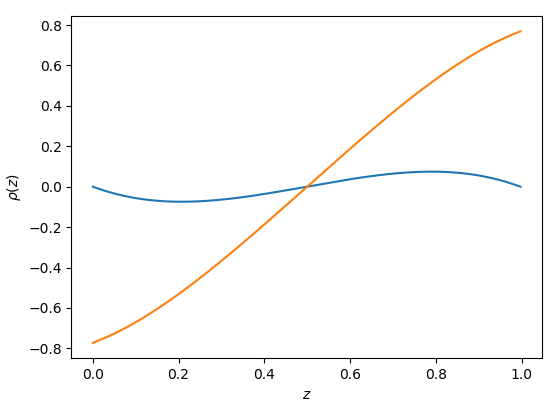
\includegraphics[width=0.9\textwidth]{figures/renormalization_comparison_rho.png}
%	    	    \end{figure}
%	    \end{column}
%	    \begin{column}{0.5\textwidth}
%		    The induced charge density $\rho$ resulting from the two different renormalization techniques with Dirichlet boundary conditions. $m=0$, $\lambda=5$.
%		    \begin{itemize}
%		    	\item \textcolor{orange}{In orange}, the charge density $\rho$ calculated through the mode sum formula.
%			\item \textcolor{blue}{In blue}, the charge density $\rho$ calculated through Hadamard point-splitting. 
%		    \end{itemize}
%		    
%	    \end{column}
%	\end{columns}
%	    \end{frame}

\begin{frame}{Closing the loop}
		
\begin{tikzpicture}[
    box/.style = {draw, rectangle, minimum width=2cm, minimum height=1cm},
    arrow/.style = {->, thin, >=Stealth},
    curved arrow/.style = {->, thick, >=Stealth, bend left}
]
\begin{centering}
	

% Nodes
\node[box] (A0) {$A_0^{(\kappa=0)}$};
\node[box, right=1cm of A0] (phi) {$\phi$};
\node[box, above right=1cm and 2cm of phi] (rho) {$\rho$};
\node[box, below right=1cm and 2cm of phi] (tildeA0) {$A^{\phi}_0^{\left( \kappa \right) }$};

% Curved arrows for the loop
\draw[arrow] (A0) -- (phi);
\draw[curved arrow, red] (phi) to[out=45, in=135] (rho);
\draw[curved arrow, red] (rho) to[out=45, in=135] (tildeA0);
\draw[curved arrow, red] (tildeA0) to[out=45, in=135] (phi);

% Center arrow with text
\node[right=0.9cm of phi] (kappa) {$\kappa \to \infty$};
 \draw[arrow, blue] (6.5, -0.25) arc [start angle=345, end angle=15, radius=1cm];


\end{centering}\end{tikzpicture}

\end{frame}

\begin{frame}{Closing the loop}
\begin{align*}
			&\left(
				\left[ 
			\omega^{ \kappa+1  }_n 
	-e A_0^{\kappa} (z)  \right]^2 
	+ \frac{d^2}{dz^2} - m^2  \right)
	\phi^{ \kappa + 1  }_n = 0 \\
			       & A_0  ^{\kappa}(z) = -\lambda \left(z-\frac{1}{2}\right) -\int_{\frac{1}{2}}^{z} \int_{0}^{z'} \rho^{\kappa}(z'')dz''   dz'
.
\end{align*}
\uncover<2->{
    \begin{themedTitleBlock}{As a fixed point problem}
	   Reminiscent of fixed point problems 
	    \begin{align*}
	    	A_0^{\kappa + 1} = f(A_0^{\kappa} )
	    \end{align*}

    \end{themedTitleBlock}	
}
\end{frame}

\section*{Fixed point problems}
\begin{frame}{Fixed point problems}
	\uncover<1->{
	    \begin{themedTitleBlock}{Definition}
	    	For $X$ a metric space, a fixed point $x\in X$ of a function $ f: X &\rightarrow X  $ is defined as $$x = f(x).$$
	    \end{themedTitleBlock}
	}
	
	\uncover<2->{
\begin{align*}
	f(A_0) = A_\text{background} + A_{induced}(A_0)
\end{align*}	    
	}

	\uncover<3->{
\begin{figure}[ht]
    \centering
    \incfig{the-function-f-as-a-black-box}
    \caption{The function f as a black box}
    \label{fig:the-function-f-as-a-black-box}
\end{figure}
	}
\end{frame}

\begin{frame}{Fixed point problems}
	    \begin{themedTitleBlock}{Definition}
	    	For $X$ a metric space, a fixed point $x\in X$ of a function $ f: X &\rightarrow X  $ is defined as $$x = f(x).$$
	    \end{themedTitleBlock}
	
\begin{align*}
	f(A_0) = A_\text{background} + A_{induced}(A_0)
\end{align*}	    

\begin{figure}[ht]
    \centering
    \incfig{the-inside-of-the-black-box}
    \caption{The inside of the black box}
    \label{fig:the-inside-of-the-black-box}
\end{figure}
\end{frame}

\begin{frame}{One dimensional fixed point problems}
	\begin{columns}
	    \begin{column}{0.5\textwidth}
		    \begin{themedTitleBlock}{Fixed point}
			    Find, if it exists 
			    \begin{align*}
				    \lim_{n \to \infty} f^{n}(x), f^{n}:= \underbrace{f \circ\ldots \circ f}_\text{n times} 
			    \end{align*}
	    \end{themedTitleBlock}
	    \end{column}
	    
	    \begin{column}{0.5\textwidth}
		    \uncover<2->{
		        \begin{figure}[ht]
			    \centering
			    \incfig{iterations-in-fixed-point-problems1}
			    \caption{Iterations in fixed point problems}
			    \label{fig:iterations-in-fixed-point-problems}
			\end{figure}
		    }
		    
	    
	    \end{column}
	\end{columns}
\end{frame}
\begin{frame}{One dimensional fixed point problems}
	\begin{columns}
	    \begin{column}{0.5\textwidth}
		    \begin{themedTitleBlock}{Fixed point}
			    Find, if it exists 
			    \begin{align*}
				    \lim_{n \to \infty} f^{n}(x), f^{n}:= \underbrace{f \circ\ldots \circ f}_\text{n times} 
			    \end{align*}
	    \end{themedTitleBlock}
	    \end{column}
	    
	    \begin{column}{0.5\textwidth}
\begin{figure}[ht]
    \centering
    \incfig{iterations-in-fixed-point-problems2}
    \caption{Iterations in fixed point problems}
    \label{fig:iterations-in-fixed-point-problems}
\end{figure}
	    
	    \end{column}
	\end{columns}
\end{frame}
\begin{frame}{One dimensional fixed point problems}
	\begin{columns}
	    \begin{column}{0.5\textwidth}
		    \begin{themedTitleBlock}{Fixed point}
			    Find, if it exists 
			    \begin{align*}
				    \lim_{n \to \infty} f^{n}(x), f^{n}:= \underbrace{f \circ\ldots \circ f}_\text{n times} 
			    \end{align*}
	    \end{themedTitleBlock}
	    \end{column}
	    
	    \begin{column}{0.5\textwidth}
\begin{figure}[ht]
    \centering
    \incfig{iterations-in-fixed-point-problems2}
    \caption{Iterations in fixed point problems}
    \label{fig:iterations-in-fixed-point-problems}
\end{figure}
	    
	   \end{column}
	   \end{columns}
   \end{frame}
\begin{frame}{One dimensional fixed point problems}
	\begin{columns}
	    \begin{column}{0.5\textwidth}
		    \begin{themedTitleBlock}{Fixed point}
			    Find, if it exists 
			    \begin{align*}
				    \lim_{n \to \infty} f^{n}(x), f^{n}:= \underbrace{f \circ\ldots \circ f}_\text{n times} 
			    \end{align*}
	    \end{themedTitleBlock}
	    \end{column}
	    
	    \begin{column}{0.5\textwidth}
\begin{figure}[ht]
    \centering
    \incfig{iterations-in-fixed-point-problems3}
    \caption{Iterations in fixed point problems}
    \label{fig:iterations-in-fixed-point-problems}
\end{figure}
	    
	   \end{column}
	   \end{columns}
   \end{frame}
\begin{frame}{The relaxing update rule}
To avoid numerical instabilities due to $\Delta \lambda$ being too big,  
\begin{align*}
	A_0^{\kappa+1} = c A_0^\kappa + (1-c)(A_\text{background}  + A^{\kappa}_\text{induced}), \hfill 0 < c \lesssim  1
\end{align*}
\end{frame}
